\section{Differential Privacy for Time Series Release}\label{sec5}
Time series release aims to publicly share private time series while preserving privacy. Value perturbation methods add noise to the data values, often using sampling and adaptive budget allocation for utility. While temporal perturbation methods dispatch elements across timestamps to obfuscate event timings, avoiding value distortion but risking empty releases or collisions.

\subsection{Value Perturbation Based Methods}
Time series release aims to directly publicize the time series for downstream tasks. Since time series release focuses on preserving the accuracy of values, privacy budget allocation is critical for controlling added noise and minimizing distortion. Therefore, a sampling-based method is often employed to select crucial elements according to the tasks, reducing the number of points requiring privacy budget allocation and enhancing utility. Additionally, to further improve the utility of the released data, a post-processing step can be adopted to correct the noisy data using prior knowledge. The outline of time series release is summarized in Fig.~\ref{release_process}.
\begin{figure}[h]
	\centering
	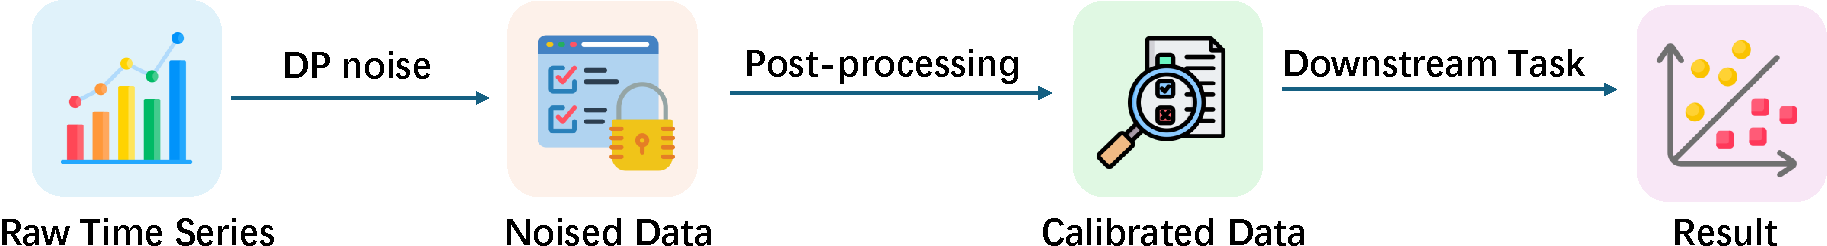
\includegraphics[width=0.8\textwidth]{submissions/submission4/figs/05-release/data_release-crop.pdf}
	\caption{The outline of time series release under differential privacy.}
	\label{release_process}
\end{figure}

\subsubsection{Privacy Budget Allocation Strategies}
User-level privacy protects the elements from any user but requires a larger privacy budget for reasonable utility, particularly challenging for time series release. Conversely, event-level privacy safeguards individual elements, yet may not suffice for comprehensive privacy guarantees. To balance the privacy levels,  
Kellaris et al.~\cite{Kellaris14} first proposed $w$-event level privacy under CDP. By leveraging $w$-event level privacy, sanitized time series can offer better privacy guarantees than event-level privacy and higher utility than user-level privacy. To optimize the advantages of $w$-event level privacy, Kellaris et al. \cite{Kellaris14} proposed two privacy budget allocation strategies. Building upon the ideas of the budget distribution and absorption strategies in \cite{Kellaris14}, Ren et al.~\cite{ren2022ldp} proposed corresponding strategies under LDP framework. To mitigate the utility degradation caused by dividing the privacy budget, the authors divide the users instead, with each user reporting only one timestamp within a $w$-length window. 
Several sampling-based methods have been developed to reduce the number of elements requiring a privacy budget, with adaptive budget allocation based on element importance. 
Wang et al.~\cite{wang2016rescuedp} introduced RescueDP, a scheme for real-time publishing of spatio-temporal crowd-sourced data with $w$-event level CDP, integrating adaptive sampling, privacy budget allocation, dynamic grouping, perturbation, and filtering techniques. The adaptive sampling component adjusts sampling rates based on data changes, ensuring efficient resource utilization. The privacy budget allocation mechanism dynamically distributes the privacy budget for sampling points across successive timestamps. Zhang et al.~\cite{zhang2017re} proposed Re-DPoctor, a real-time health data releasing scheme ensuring $w$-event level CDP, enhancing utility with a partition algorithm safeguarding health data patterns and improving privacy through adaptive sampling and budget allocation.
He et al.~\cite{he2022ordinal} introduced a new privacy concept using condensed local differential privacy (CLDP)~\cite{gursoy2019secure} for $w$-event level privacy, aiming to enhance utility. They save privacy budget from empty releases and reallocate it to released elements, and utilize a PID controller-based method for adaptive budget allocation. However, this approach may inadvertently disclose private information through omitted empty points.

\subsubsection{Optimization Strategies}
Leveraging the correlations present in time series, the pre-processing or post-processing methods can be applied to improve the utility of the perturbed data.
Ren et al.~\cite{ren2018textsf} addressed privacy challenges in high-dimensional crowdsourced data by proposing LoPub, an LDP data publication algorithm under event-level privacy. They use expectation maximization (EM) and Lasso regression to efficiently estimate multivariate joint distributions, identifying attribute correlations to reduce data dimensionality for distribution learning speed and utility improvements.
Wang et al.~\cite{wang2019locally} proposed the methods, LoCop and DR\_LoCop, for releasing high-dimensional crowdsourced data under event-level LDP. The methods comprise four integrated components: a transformation component that ensures LDP by hashing and randomizing the data, an estimation component that infers probability distributions from the resulting Bloom filter strings, a computation component that derives marginal distributions and captures dependencies among dimensions, and a sampling component that generates a new synthetic dataset based on the computed distributions and dependencies. 
Fioretto and Hentenryck~\cite{fioretto2019optstream} introduced OptStream,  a method for releasing time series under $w$-event level, which extends to handling hierarchical streams like energy profiles, making it applicable beyond its original energy domain. OptStream involves four key steps: sampling points for private measurement, perturbing them for privacy, reconstructing non-sampled points, and post-processing with convex optimization to improve accuracy by redistributing added noise.
Zhang et al.~\cite{zhang2022differentially} introduced a method for releasing differentially private sequential data using first-order autoregressive processes under user-level privacy. Their approach estimates unreleased data from previously released data by leveraging learned correlations, without requiring prior knowledge. The estimated data is combined with the observed data and perturbed with calibrated noise at each timestamp, facilitating real-time data release.
Li et al.~\cite{li2023locally} proposed a framework for locally private stream data release that employs shuffling and subsampling techniques. Their approach maintains utility in the context of continual data collection by sampling a subset of users at each timestamp. An optimal sample size is determined to reduce redundant data and enhance utility, and the framework incorporates pre-processing within the shuffler to mitigate bias arising from distributed sampling. 
Besides pre- or post-processing methods, Bao et al.~\cite{bao2021cgm} proposed a mechanism based on the assumption of data fluctuation. Since time series may not change significantly over time, this mechanism formalizes the correlation between elements, allowing a later element to be represented by previous elements. To protect privacy, noise is added to the correlation.

\subsection{Synthesis Based Methods}
Directly releasing users' data poses significant risks of privacy breaches. An alternative approach is to train a synthesis model under strict privacy conditions and then release the data generated by this model for downstream tasks. To synthesize time series data under DP, one method involves first estimating the relevant statistics and then generating the synthetic data based on these estimations. Additionally, the advent of Generative Adversarial Networks (GANs) under DP~\cite{xie2018differentially, jordon2018pate} has facilitated the use of deep learning algorithms to generate data, thereby enhancing both privacy protection and data accuracy.

\subsubsection{Synthesis Based on Statistics}
Synthesis mechanisms based on statistical features first capture the statistical characteristics from datasets under DP. Subsequently, new data is generated according to these estimated statistics. He et al.~\cite{he2024online} introduced an efficient polynomial-time algorithm for generating online differentially private synthetic data under event-level privacy from a continuous time series within the hypercube $[0, 1]^d$. The algorithm achieves near-optimal accuracy bounds in $1$-Wasserstein distance and extends previous work to include Lipschitz queries. By utilizing an online hierarchical partitioning approach and a novel Inhomogeneous Sparse Counting Algorithm, the method maintains strong privacy guarantees while ensuring high utility for infinite time horizons. To achieve a higher privacy level, 
Bun et al.~\cite{bun2024continual} focused on generating differentially private synthetic data through statistical estimation under user-level CDP. They proposed algorithms that maintain the accuracy of fixed time window and cumulative time queries, ensuring minimal error while preserving privacy. Their approach involves a two-stage process that combines noisy estimates with post-processing techniques to ensure consistency and accuracy in synthetic data generation.



% GAN
\subsubsection{Synthesis Based on Generative Models}
In addition to statistics-based mechanisms, another method for synthesizing time series is through Generative Adversarial Networks (GANs). Unlike other data types, time series requires consideration of temporal correlations. 
Frigerio et al.~\cite{frigerio2019differentially} presented a framework for releasing high-quality open data while ensuring user privacy through DP, addressing both continuous and discrete data. By leveraging deep learning and generative models with long short-term memory networks, the framework maintains data utility and correlations, introducing innovations such as clipping decay to optimize performance.
Wang et al.~\cite{wang2020part} introduced PART-GAN, a privacy-preserving generative model designed for time series augmentation and sharing. PART-GAN combines Conditional and Temporal Generative Adversarial Networks (CT-GAN) with differential privacy mechanisms, enabling the generation of unlimited synthetic data that addresses issues of incomplete and irregularly sampled time series.
Torfi et al.~\cite{torfi2022differentially} proposed a mechanism to generate high-quality synthetic health record data while ensuring privacy using R\'enyi Differential Privacy (RDP). Their framework combines convolutional autoencoders and convolutional generative adversarial networks (CGAN) to effectively handle both discrete and continuous data, preserving temporal and feature correlations.
For specific applications, Lamp et al.~\cite{lamp2024glucosynth} introduced GlucoSynth, a novel privacy-preserving GAN framework designed to generate high-quality synthetic glucose traces while maintaining strong differential privacy guarantees. By focusing on preserving the relationships among glucose events (motifs) and temporal dynamics, GlucoSynth addresses the unique challenges of synthesizing glucose data.





\subsection{Discussion}
The aforementioned release mechanisms modify the values of the original time series, which can degrade utility in value-critical scenarios. For elements in a time series where occurrence indicates more sensitive information, temporal perturbation can be employed to avoid distorting the original values. Ye et al.~\cite{ye2021beyond} first proposed a method to achieve temporal perturbation in the local setting, maintaining the privacy guarantee while enhancing utility.
\begin{figure}[htbp]
	\centering
	\begin{minipage}{0.4\textwidth}
		\centering
		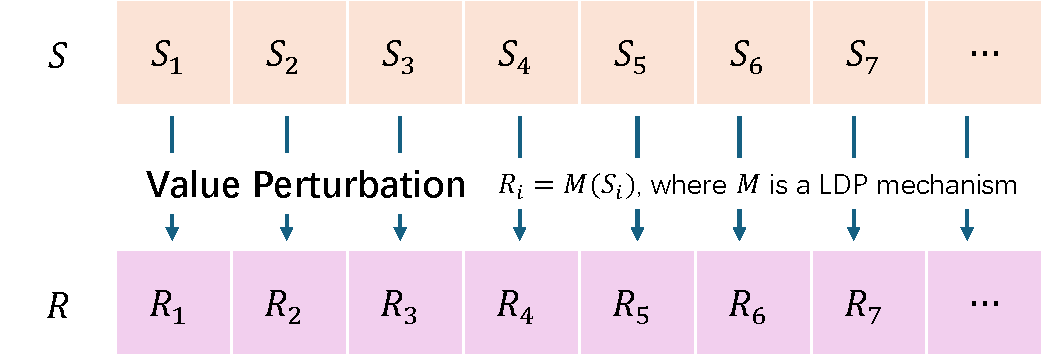
\includegraphics[width=\linewidth]{submissions/submission4/figs/05-release/value_perturbation-crop.pdf}
	\end{minipage}\hspace{0.55in}
	\begin{minipage}{0.4\textwidth}
		\centering
		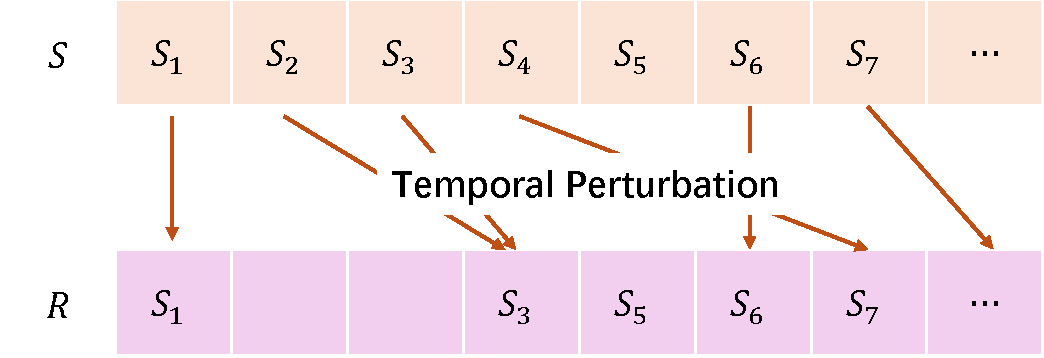
\includegraphics[width=\linewidth]{submissions/submission4/figs/05-release/temporal_perturbation-crop.pdf}
	\end{minipage}
	\caption{Value perturbation-based methods will perturb the original values by adding DP noise. In contrast, temporal perturbation-based methods will dispatch the values to corresponding timestamps for release.}
	\label{vptp}
\end{figure}
As illustrated in Fig.~\ref{vptp}, unlike value perturbation that directly modifies the original values by adding LDP noise, temporal perturbation dispatches elements across different timestamps. This obfuscates the precise occurrence times, preventing adversaries from determining the exact event timings. However, temporal perturbation can lead to issues such as delayed releases, empty releases (where no elements are dispatched to certain timestamps), and element substitutions, resulting in missing data.  To address these issues,  Ye et al.~\cite{ye2023stateful} proposed a bi-directional perturbation mechanism that eliminates collisions during the dispatching process, ensuring that elements are only delayed. Furthermore, Mao et al.~\cite{mao2023utility} extended the definition to a metric-based version tailored for anomaly detection, aiming to reduce collisions involving anomalous elements.  However, these proposed mechanisms~\cite{ye2021beyond, ye2023stateful, mao2023utility} primarily address event-level privacy concerns, leaving room for enhancements to achieve higher levels of privacy.




















